% !TeX spellcheck = es_ES

\title{Adaptaci�n y extensi�n de la herramienta de captura y an�lisis de tr�fico Ksensor\\Dise�o de alto nivel}
\author{Javier Domingo Cansino}

\documentclass[11pt,a4paper]{report} % Para tener un documento grande pero sin ser un libro (solo hay esta posibilidad)
\usepackage[latin1]{inputenc}   % Para la codificaci�n
\usepackage{textcomp}           % Para los simbolos de euro
\usepackage[spanish]{babel}     % Para el lenguaje que tenga bien
\usepackage[T1]{fontenc}        %      los saltos de linea con gui�n etc.
\bibliographystyle{alpha}       % Estilo de bibliograf�a
\usepackage{graphicx}           % Para insertar im�genes
\graphicspath{{../images/}}     % La ruta relativa de las im�genes
\usepackage{hyperref}           % Hacer links guays entre secciones y hacia fuera
\usepackage[hypcap]{caption}    % Hacer que las referencias se vean, y no se queden por encima (referenciando imagenes, etc.)
\hypersetup{
	colorlinks=true,
	linkcolor=blue,
	citecolor=red,
}
\usepackage[table]{xcolor}      % Dar colores a las tablas
\usepackage{eurosym}            % para tener el simbolo del euro
\usepackage{setspace}           % Para hacer el espaciado entre l�neas
\setstretch{1.4}                %      1.4 del espacio normal
\usepackage{parskip}            % El espaciado entre parrafos 
\setlength{\parindent}{25pt}    %      lo ponemos a 25pt
\usepackage[margin=3cm]{geometry} % Cambiar el margen del texto

\usepackage{fancyhdr}           % Cambiar las cabeceras del documento
\pagestyle{fancy}               %      y usar los cambios
\lhead{
\includegraphics[width=5cm]{ingenieros-bilbao}}
\rhead{Adaptaci�n y extensi�n de la herramienta\\ de captura y an�lisis de tr�fico Ksensor}
\cfoot{\thepage}
\setlength{\headheight}{47pt}

\usepackage{titlesec}           % cambiar el estilo soso de los cap�tulos
\titleformat{\chapter}[hang]{\Huge\bfseries}{\thechapter. }{0pt}{\Huge\bfseries}
\usepackage{makeidx}            % Hacer �ndices

% % % % % % % % % % % % % % % % % % % % % % %
% Secci�n de comandos personalizados        %
% % % % % % % % % % % % % % % % % % % % % % %
\newcommand{\reference}[2]{\hyperref[#1]{\textit{\ref*{#1} #2}}}
\makeindex

\begin{document}
\pagenumbering{Roman}
\maketitle % Crear el t�tulo
\tableofcontents % Crear la tabla de contenidos

\pagenumbering{arabic}

% !TeX spellcheck = es_ES
% !TeX root = main.tex

\chapter{Introducci�n}

En los �ltimos a�os, las tecnolog�as inform�ticas de la comunicaci�n est�n revolucionando la manera de comunicarse del mundo entero. Tener acceso a Internet se ha convertido en algo necesario para poder ponerse en contacto con el resto del mundo.

Cada vez hay m�s dispositivos conectados, con el consiguiente crecimiento del tr�fico en todas las redes. Incluso empresas que antes contrataban redes privadas para sus comunicaciones, ahora utilizan Internet para interconectar sus redes.

Como en cualquier servicio cr�tico el mantenimiento debe ser proactivo y por ello se han creado m�todos para garantizar la m�xima eficiencia de las comunicaciones. Para ello se debe garantizar la seguridad en la red y la detecci�n instant�nea de problemas, asegurando as� la \textit{QoS} (\textit{Quality of Service}, Calidad de Servicio).

Para la securizaci�n de la red se implantan \textit{firewalls}, \textit{proxys}, e \textit{IDS}s (\textit{Intrusion Detection System}, Sistema de Detecci�n de Intrusi�n), que se encargan de evitar accesos externos no autorizados a la red, controlar el tr�fico saliente, y detectar posibles atacantes dentro de la red.

El m�todo para asegurar la calidad de las comunicaciones es la medici�n de par�metros de \textit{QoS}, tales como retardo de los paquetes, errores en la transmisi�n, tipos de tr�fico comunes, rutas �ptimas, etc.

Son varias las soluciones comerciales que implementan estos servicios pero actualmente no hay ninguna que implemente todo en un mismo sistema. Adem�s, no hay ning�n producto de c�digo libre que aproveche al m�ximo la posible eficiencia del equipo, haciendo un an�lisis \textit{online}\footnote{Online se refiere a hacer el an�lisis mientras se captura, en vez de capturar, guardar y luego analizar.}.

En el grupo de investigaci�n \textit{Network Quality and Security (NQAS)} se ha dise�ado un sonda que implementa algunas de las citadas funcionalidades. En el dise�o de la misma se ha contemplado la posibilidad de m�s adelante poder ampliarlo de una manera sencilla. Como valor a�adido fundamental, aprovecha al m�ximo los recursos disponibles, ya que ha sido programado de una manera que permita ejecuci�n multi-hilo.

Este prototipo se llama ksensor\cite{KABO05}, aunque no es el primero que se ha creado. La l�nea de investigaci�n principal, llamada hi-sensor, ha ido haciendo cada vez m�s complejo el dise�o y la programaci�n del prototipo con el objetivo de mejorar la eficacia.

A grandes rasgos, primero se dise�� de forma que la aplicaci�n fuera un programa de usuario que capturaba a trav�s de una librer�a est�ndar para la captura de paquetes de forma promiscua. Se utilizaron tambi�n las librer�as para tener computaci�n multi-hilo, y se consiguieron unos resultados prometedores.

Cuando se empezaron a analizar redes de alta velocidad en saturaci�n se vio que hab�a un problema: El equipo estaba continuamente capturando, y no hab�a espacio para el an�lisis. Para solucionar este problema, se migr� a espacio de kernel.

El kernel es la base que hace que todos los programas funcionen. Es un programa que se encarga de gestionar los dispositivos y recursos del ordenador para ofrecer una interfaz libre de detalles a los programas. Adem�s, tambi�n se encarga de hacer que varios programas se ejecuten de una manera que proporcione a todos y cada uno la forma de parecer que est�n en ejecuci�n continua. A parte de eso, se encarga de que los programas sean capaces de hacer un direccionamiento virtual de una forma transparente a ellos, manejando eficazmente una MMU (\textit{Memory Management Unit}, Unidad de Gesti�n de Memoria), de manera que permite que estos sea posible compilarlos como si solo fueran a existir ellos.

En general, del dise�o de un buen kernel depender� la eficiencia del sistema. En nuestro caso, el dise�o del kernel no est� hecho para nuestro tipo de sistema, una sonda de tr�fico, pero a trav�s de una serie de modificaciones, podemos cambiar el comportamiento del sistema para amoldarlo a nuestro caso de uso. Todo sea dicho, la eficiencia del kernel actual es buena para los sistemas operativos de car�cter general, en los que capturar los paquetes de uno mismo es suficiente, y que es una cantidad peque�a en comparaci�n con el tr�fico de la red.

El cometido del sistema que queremos es �nicamente para capturar y procesar paquetes y por lo tanto, la m�xima eficiencia se puede describir como el equilibrio entre el tiempo en el que el ordenador esta capturando y el que est� analizando. Se tienen que capturar exactamente el n�mero de paquetes que se van a analizar.

La implementaci�n actual del sistema ha quedado obsoleta para kernels actuales, ya que el tratamiento de los paquetes se hace de una forma diferente. Ahora se crean \textit{superpaquetes} ensamblando desde la captura los paquetes que tienen una serie de par�metros iguales, como pueden ser la IP de origen, IP de destino, puerto TCP destino y origen. De esta manera, al pasar un �nico paquete (aunque grande) a la pila de protocolos, se acelera su tratamiento, ya que las copias de los paquetes se pueden hacer en una �nica transacci�n.

Por lo tanto, el proyecto se enfoca a mejorar el anterior dise�o para adaptarlo a la nueva manera de hacer las cosas, crear una serie de herramientas para validar el dise�o y adaptar el proyecto a los est�ndares defacto existentes en kernel.org para hacer posible la liberaci�n p�blica del c�digo. La tarea de mayor relevancia en estos momentos es posibilitar un estudio comparativo entre un sistema normal y la aplicaci�n.
\chapter{Arquitectura general}

En este cap�tulo se describe la arquitectura general del sistema propuesto en el presente proyecto. Como el dise�o anterior se ha considerado v�lido en el entorno de pruebas, adem�s obteniendo muy buenos resultados, en esta secci�n se explicar�n los cambios puntuales que ser�n necesarios para hacer que el anterior dise�o siga funcionando.

Este dise�o, adem�s contemplar� los m�dulos complementarios creados en este proyecto y la organizaci�n de los mismos.

\section{Arquitectura en espacio de kernel}
Una de las primeras decisiones de dise�o que hay que hacer es la elecci�n de la versi�n a la que se va a migrar. Seg�n lo que se ha analizado, la interfaz hacia los m�dulos y drivers de kernel se ha mantenido de la misma forma, permitiendo as� que el trabajo de migraci�n para Ksensor se integre de una forma sencilla.

El principal problema de la migraci�n de Ksensor son las funciones espec�ficas que se han implementado para su correcto funcionamiento, las cuales utilizan estructuras internas normalmente no visibles para los m�dulos, lo que hace que sean incompatibles.

A continuaci�n, se intentar�n explicar las diferencias conceptuales entre el kernel 2.6.15 y 3.6 en los puntos relevantes para nuestra implementaci�n:
\begin{itemize}
\item Estrategia de captura de paquetes
\end{itemize}

\subsection{Estrategia de captura de paquetes}
Existen diferentes estrategias para capturar el tr�fico de red, cada cual con sus
ventajas e inconvenientes:

\begin{description}
\item [Captura basada en interrupciones]
Este mecanismo es el m�s sencillo, pero tambi�n el m�s ineficiente. Cada vez que llega un paquete a la tarjeta de red, �sta genera una interrupci�n y se ejecuta la rutina de atenci�n correspondiente. En esta rutina se captura el paquete y se encola para un posterior procesamiento por parte del subsistema de red del kernel. Este proceso se repite con cada paquete que llega a la tarjeta.

La mayor ventaja de este mecanismo es la baja latencia con la que se reciben los paquetes. Sin embargo, tiene un grave inconveniente. A medida que la frecuencia de llegada de paquetes al sistema crece, se consumen cada vez m�s recursos de la CPU para atender las interrupciones que se generan. Si el ratio de llegada crece a�n m�s, la captura de paquetes puede llegar a monopolizar la CPU, impidiendo que se ejecute cualquier otra tarea y llegando a lo que en \cite{JMKR96} se denomin� como livelock.

\item[Captura basada en polling]
Para evitar los livelocks se pueden emplear mecanismos de polling, es decir, se pregunta peri�dicamente a la tarjeta si ha llegado alg�n paquete, en cuyo caso se capturan todos los que hayan llegado hasta ese momento. De este modo, a�n si la tasa de llegada de los paquetes es muy alta, el sistema operativo podr� controlar el consumo computacional que se dedica al proceso de captura. Sin embargo, esta estrategia tambi�n presenta algunos inconvenientes, ya que si la tasa de llegada es baja, se estar� interrogando a la tarjeta de red a pesar de que no haya llegado ning�n paquete, consumiendo recursos de forma innecesaria. Adem�s, la latencia con la que se reciben los paquetes es mayor.

\item[Captura mixta]
Dadas las ventajas e inconvenientes de las t�cnicas anteriores, en \cite{JMKR96} se propuso un mecanismo mixto en el que se trataba de evitar los livelock a la vez que se reduc�a el consumo innecesario debido al polling. Para ello, utiliz� una t�cnica llamada coalescencia de interrupciones.

Cuando llega el primer paquete, se produce una interrupci�n hardware y se ejecuta la rutina de atenci�n correspondiente a esa interrupci�n. En esta rutina se notifica al sistema acerca de la llegada de nuevos paquetes que necesitan ser recogidos, y a continuaci�n se deshabilitan las interrupciones. Cuando el sistema lo considere oportuno, se ejecutar� la tarea del kernel encargada de la recepci�n de paquetes, que har� un polling sobre la tarjeta de red mientras sigan llegando paquetes.

Finalmente, se vuelven a habilitar las interrupciones. De esta manera, si la tasa de llegada es baja, el sistema se comporta como un sistema basado en interrupciones, y si aumenta, se capturan m�s paquetes por interrupci�n, asemej�ndose a un sistema basado en polling.
\end{description}

\chapter{Arquitectura de Ksensor}
El dise�o actual de Ksensor debe ser adaptado para utilizar la nueva manera de gestionar la captura del kernel de Linux. Este dise�o comprende principalmente modificaciones en el dise�o de bajo nivel, por lo que se dejar� para el documento que compete.

Ya se han explicado los cambios del sistema en la anterior interfaz, por lo que aqu� se mencionar�n las funcionalidades espec�ficas que utilizaban la interfaz antigua a reemplazar.

\section{Necesidades}

Las funcionalidades que Ksensor necesita del kernel se han dividido por las zonas a las que pertenecen del sistema. Tanto como conceptualmente pueden ser parecidas, se separan para que en el dise�o de bajo nivel se entiendan de donde viene cada uno de los nuevos dise�os.

\subsection{Tener lista de interfaces de captura.}

El sistema Ksensor debe ser utilizado �nicamente para los paquetes que se capturen desde las interfaces configuradas para tal efecto, y como tal, el sistema debe tener una lista de las interfaces a las que debe controlar.

La interfaz interna para la gesti�n de listas no ha cambiado, ya que como se mencionaba antes, durante el desarrollo del kernel, se ha intentado dejar el interfaz hacia los m�dulos lo m�s inmutable posible. En ese aspecto la funcionalidad requerida tiene la misma forma de acceso.

\subsection{Discriminar paquetes por interfaz}

En la implementaci�n anterior, la funcionalidad utilizaba una referencia interna del paquete hacia la interfaz. En este caso, con los cambios en el tratamiento de paquetes, debemos tener en cuenta que ahora las entradas en el sistema son virtuales y que las interfaces de red no son representadas de la misma manera.

Ahora las interfaces f�sicas han dejado de ser gestionadas en el polling, y se gestionan las bocas o colas de entrada de las que disponga la tarjeta. El rendimiento de captura se ver� afectado por lo tanto por las interrupciones de la tarjeta, y no por las recepciones en una sola interfaz.

Ksensor debe ser por lo tanto pensado para gestionar todos los paquetes que lleguen a una tarjeta de red, ya que no se puede aplicar un control de flujo efectivo a solo una interfaz. De todos modos, aunque se gestione una NIC entera, se puede elegir de cual(es) se procesar�n los paquetes, aunque el resto de interfaces de la tarjeta no se puede asegurar tengan el procesado necesario.

\subsection{Establecer la afinidad entre interfaces y procesadores.}

Antes, como las tarjetas ten�an un �nico interfaz, no hab�a mayores dificultades con esta necesidad. Ahora se deben gestionar las interfaces dependiendo de a qu� tarjeta pertenezcan. Tambi�n ha cambiado el m�todo para establecer la afinidad en sistemas multiprocesamiento, y habr� que adaptar las llamadas correspondientes para ello.

\subsection{Activar o desactivar la captura de paquetes en el sistema.}

Al haber separado la captura de la gesti�n de la interfaz, el �nico m�todo para desactivar la captura de una interfaz es la de desactivarla para toda la tarjeta de red. Por lo tanto se debe volver a adaptar la manera en la que ksensor limita la captura de paquetes.


\section{Mejoras}
Aqu� se mencionar�n las mejoras de dise�o que se han pensado para Ksensor, donde las modificaciones se justifican a trav�s de los efectos vistos en las pruebas.

\subsection{Control de congesti�n}

Actualmente, el sistema de control de congesti�n es la opci�n de configuraci�n que m�s rendimiento ofrece al sistema, se encarga de evitar la captura de m�s paquetes de los necesarios, y asegura un equilibrio entre la captura y el procesamiento.

Este sistema funciona tal y como est� descrito en el documento de dise�o de alto nivel de \cite{KABO05}. El funcionamiento es simple, una vez la cola de captura de Ksensor se llena, este deja de capturar hasta que los procesos de an�lisis del mismo dejan la cola a la mitad de su capacidad. Desde ese momento, el proceso de captura se vuelve a activar, y vuelve a llenar la cola.

Como se puede observar, la captura de paquetes variar� en forma de diente de sierra, y podr�a ocasionar, que en caso de que el sistema se enfrentara a tasas de tr�fico cerca de su saturaci�n, dejara de capturar algunos paquetes por su llegada al m�ximo, y se perder�an todos aquellos paquetes, que a�n teniendo sitio despu�s de la saturaci�n, se perder�an por este par�metro est�tico.

La soluci�n que se pretende adquirir en esta nueva implementaci�n es que la cola est� el m�ximo tiempo posible en saturaci�n, sin dejar de lado la eficacia. Una softirq, tiene como objetivo capturar un n�mero m�ximo de paquetes definido, 300, en un m�ximo de tiempo, 2 \textit{jiffies}.

El dise�o que se va a seguir, va a dar resultado a gr�ficas en forma de diente de sierra, pero se van a distribuir las capturas para ir llenando la cola siempre que se llegue al nivel de $tama\check{n}o\ de\ cola- 300$. Este cambio de dise�o se espera justificar con pruebas contra el dise�o alternativo.

\subsection{Bloqueos en secciones cr�ticas}

Ksensor, al contrario de lo que se pensaba, no es tan �ptimo como se pensaba en computadoras multin�cleo de gran potencia. Tras un an�lisis del c�digo, se han podido identificar varios segmentos del mismo que hay secciones cr�ticas demasiado grandes, e incluso, secciones cr�ticas que no son necesarias por el dise�o del sistema.

Uno de los mayores problemas que se ha podido discernir es la situaci�n de bloqueo que se da en el acceso a la cola �nica de procesamiento de las arquitecturas multiprocesador, donde hay varias instancias que se quedan a la espera de conseguir acceso a la cola.

Tanto como en el proyecto de Ksensor \cite{KABO05} hay un desarrollo argumentado muy completo de porqu� utilizar una cola es lo �ptimo, no se entra a debatir sobre la posibilidad de procesar paquetes en grupos, tal y como hace el nuevo m�todo GRO \ref{sec:gro}.

\subsubsection{Mejoras}
Uno de los cambios de dise�o en Ksensor es la asignaci�n variable de cupos de paquetes. Una instancia, que por el motivo que fuera se queda bloqueada en el acceso a la cola, coger� un paquete m�s cada vez que se quede bloqueado al intentar acceder a la cola.

Es importante especificar que el dise�o que se plantea no tiene como objetivo que un hilo de Ksensor acabe cogiendo cada vez m�s paquetes y por ello debe distinguirse entre que aumente el tiempo de bloqueo porque no hay paquetes o porque haya otras instancias intentando acceder.

Las pautas que se seguir�n en el dise�o de bajo nivel deben ser:
\begin{itemize}
\item Deber� cogerse un paquete m�s cada vez que el hilo de an�lisis se quede bloqueado por otro hilo.
\item Se coger�n hasta un m�ximo de $n\ paquetes$ por acceso a la cola, donde \\$n=n\acute{u}mero\ de\ procesadores$.
\item Se coger� un paquete menos cada vez que el hilo de an�lisis tenga un acceso sin bloqueo.
\end{itemize}

Se ha decidido limitar a esta cantidad porque es una cantidad que var�a dependiente del n�mero de agentes que intentan acceder. Con estas especificaciones del dise�o, se espera que el rendimiento sea un 10\% mayor. Este control de congesti�n se implementar� como una alternativa al control de congesti�n que ya existe para su validaci�n.

\chapter{Arquitectura del traceador}
El m�dulo de traceo es como su nombre indica un m�dulo para sacar trazas del sistema. Se puede definir traza como una referencia de como est� funcionando un determinado programa en un instante. Una caracter�stica inherente a una traza debe ser que tenga poca repercusi�n en el funcionamiento del programa, que puedan ser muchas trazas, y que se guarden el m�nimo n�mero de datos posibles.

Todo esto es lo que define 
\chapter{M�dulo de estad�sticas}

En este apartado se explicar� como se ha creado el m�dulo de estad�sticas. Es importante que se entienda que este m�dulo debe ser desarrollado para su uso en un kernel normal, aunque optativamente, si se compila con soporte para Ksensor, se a�adir�n algunas estad�sticas para este.

En este m�dulo se seguir� un orden an�logo a los anteriores, en un principio, se explicar� como se ha creado e implementado la interfaz hacia el usuario, a continuaci�n, se pasar� a explicar cual es la interfaz hacia el sistema, y por �ltimo, se describir� la manera en la que funciona internamente.

\section{Interfaz hacia el usuario}

Tal y como se ha explicado en el documento de dise�o de alto nivel, este m�dulo crear� una entrada en \textit{procfs} para cada una de las estad�sticas. Por lo tanto, utilizando las funciones espec�ficas de creaci�n de ficheros en procfs se crean as�.

\begin{lstlisting}[caption={Crear entrada de procfs}, label={stats-procfs}]
entry = create_proc_entry("polling_packets", 0644, iface_dir);
entry->read_proc = show_var;
entry->data = &napi->capture_stats.polling_packets;
\end{lstlisting}

Este segmento de c�digo ejemplifica la forma en la que se crea y se inicializa un fichero de proc. En la primera l�nea se crea la entrada, en la segunda se le indica la funci�n que tiene que ser llamada en caso de que el usuario quiera leer el fichero, y en la tercera se le se�ala cuales son los datos que tiene que recibir la citada funci�n.

Esta es la manera de crear todas esas entradas. Se ha dise�ado de tal manera que cree una entrada de cada estad�stica por interfaz, en el directorio \code{iface\_dir}.

Adem�s, para poder resetear las estad�sticas, se ha creado una entrada que al pasarle cualquier valor pone a cero todas las estad�sticas.

\section{Interfaz hacia el kernel}

Este m�dulo se ha creado como un m�dulo que utiliza una variable a�adida a \code{struct napi\_struct} que sirve para ir recolectando y a�adiendo las estad�sticas. Las mediciones est�n hechas a mano en el c�digo, en distintas partes. Todas las mediciones se efectuan utilizando la funci�n \code{sched\_clock}, que es la medida m�s a bajo nivel que se puede encontrar sin perder el soporte multiplataforma. Adem�s, esta medici�n tiene algunes controles que aseguran una correcta medici�n, ya que en caso de hacerlos con otras funciones, como \code{rdtscl}, se produce un kernel panic en entornos de hardirq.

Por lo tanto, una muestra de como se hace la medici�n de una hardirq es esta:

\begin{lstlisting}[caption={Medir hardirq}, label={stats-hardirq}]
static irqreturn_t hardirq_handler(int irq, void *data)
{
	unsigned long long int int_start;
	int_start=sched_clock();

	/* ... */
	
	napi.capture_stats.hardirq_num++; //increment hard interrupt
	napi.capture_stats.hardirq_ac += sched_clock() -  int_start;
	return IRQ_HANDLED;
}
\end{lstlisting}

De esta manera, como se puede observar, se est� midiendo el n�mero de hardirqs y el tiempo que tarda en cada una de ellas. Como se puede observar, es imposible no efectuar la medida, no hay ninguna manera de evitarla, por lo tanto, aunque esto sea parte de las modificaciones en el m�dulo, el m�dulo propiamente dicho solo es la interfaz hacia el usuario, y el encargado de resetear en caso de que as� lo pida el usuario.

\section{Funcionamiento interno}

Como se puede observar, el funcionamiento interno del m�dulo es sencillo, se dedica a mostrar los par�metros que se han programado, de una forma que facilita el filtrado por tipo. La verdadera dificultad en el funcionamiento es decidir donde poner las trazas y en seguir todo el flujo de kernel para medir exactamente lo que se requiere.

Este tipo de estad�sticas son totalmente personalizadas, ya que se modifica el c�digo de los drivers para sacar mediciones de su rendimiento. Aunque sea un m�dulo que se pueda ejecutar sin Ksensor, su mayor objetivo es la validaci�n de este, por ello las estad�sticas solo se han implementado para los drivers e1000, e1000e y tg3, usados en el laboratorio para las pruebas.
\chapter{Dise�o de la integraci�n}

Este es un cap�tulo que tiene como objetivo explicar con un dise�o muy superficial un trabajo que se ha desarrollado m�s en el dise�o de bajo nivel, que no entra dentro del dise�o de c�digo, sino m�s bien en la l�nea de integraci�n con los est�ndares oficiales que pretende seguir este proyecto.

\section{Integraci�n con est�ndares}

En esta secci�n se describir�n los diferentes est�ndares \textit{de-facto} con los que se quiere integrar todo el c�digo de Ksensor y el asociado a este.

\subsection{Est�ndares de directorio}

Se pretende integrar Ksensor dentro de la estructura de directorios de una forma completa. Al igual que muchos otros drivers, o partes del kernel, esto se ha hecho creando una carpeta en el directorio que m�s raz�n de pertenecer ten�a. La idea principal detr�s de este directorio es introducir en esa parte todo lo desarrollado en el grupo de investigaci�n NQaS para su posible liberaci�n.

\subsection{Est�ndar de c�digo}

Tanto como es importante la integraci�n de los ficheros que se han desarrollado en NQaS, es importante acotar las modificaciones como est� hecho en el resto del kernel. Se han acotados todas las inserciones por categor�as o secciones, que permiten compilar ciertas funcionalidades, y otras no.

Todo esto debe ser asimismo configurable para facilitar el uso de las aplicaciones, por ello, se ha integrado todo en una categor�a que permite su total desactivaci�n, NQAS dentro de la secci�n de red, y dentro se han dividido las aplicaci�n Ksensor de los m�dulos auxiliares para validarlo, y dentro de la aplicaci�n Ksensor se pueden elegir opciones de depuraci�n y estad�sticas.

Es muy importante que el dise�o en esta parte concuerde con el c�digo y con la l�gica de la aplicaci�n, ya que dejar alg�n trozo suelto podr�a ser fatal y har�a que fallara la compilaci�n. En el plan de pruebas se especificar� como comprobar que el dise�o de esta integraci�n con el est�ndar de c�digo ha sido correctamente implementado.


\section{Integraci�n en el repositorio}

Uno de los problemas a los que se enfrentaba Ksensor en caso de liberaci�n era que no utilizaba los m�todos de desarrollo de kernel, ahora que se ha integrado en el �rbol de kernel como cualquier otro componente, se tiene que integrar de una manera constantemente actualizada esta versi�n en el repositorio.

En caso de liberar el c�digo, se ha creado una rama de desarrollo paralela a la master de kernel, partiendo de la versi�n 3.6, que est� lista para su uso con un sistema de Integraci�n Continua (CI).

\chapter{Entorno de pruebas}
En este cap�tulo se presenta el entorno de pruebas de Ksensor, en el cual se han llevado a cabo las pruebas de rendimiento que permitieron evaluar la mejora de prestaciones obtenida con la adaptaci�n Ksensor.

La idea de esta secci�n es introducir los conceptos de alto nivel que se han utilizado en el proyecto anterior, y sobre las cuales se crear�n nuevas herramientas para la integraci�n de los nuevos m�dulos en el entorno de pruebas.

As� pues, primeramente se presentar� la arquitectura de pruebas existente y a continuaci�n, se describir�n todos los elementos nuevos que la componen, tanto los creados en otros proyectos \cite{DAPR10}, como los creados en este proyecto con objetivo de integrar las nuevas partes del sistema. En el documento de Dise�o de Bajo Nivel se podr� consultar una informaci�n m�s detallada .

\section{Arquitectura de pruebas}
La arquitectura de pruebas del sensor se basa en la plataforma gen�rica para la automatizaci�n de pruebas dise�ada en \cite{AABS05}, la cual permite, como su propio nombre indica, lanzar bater�as de pruebas, configurando de forma automatizada todos los agentes o elementos que participan en la misma. La arquitectura de pruebas de Ksensor se ilustra en la figura \reference{fig:arquitectura-de-pruebas}{Arquitectura de pruebas}

\begin{figure}[h]
\centering
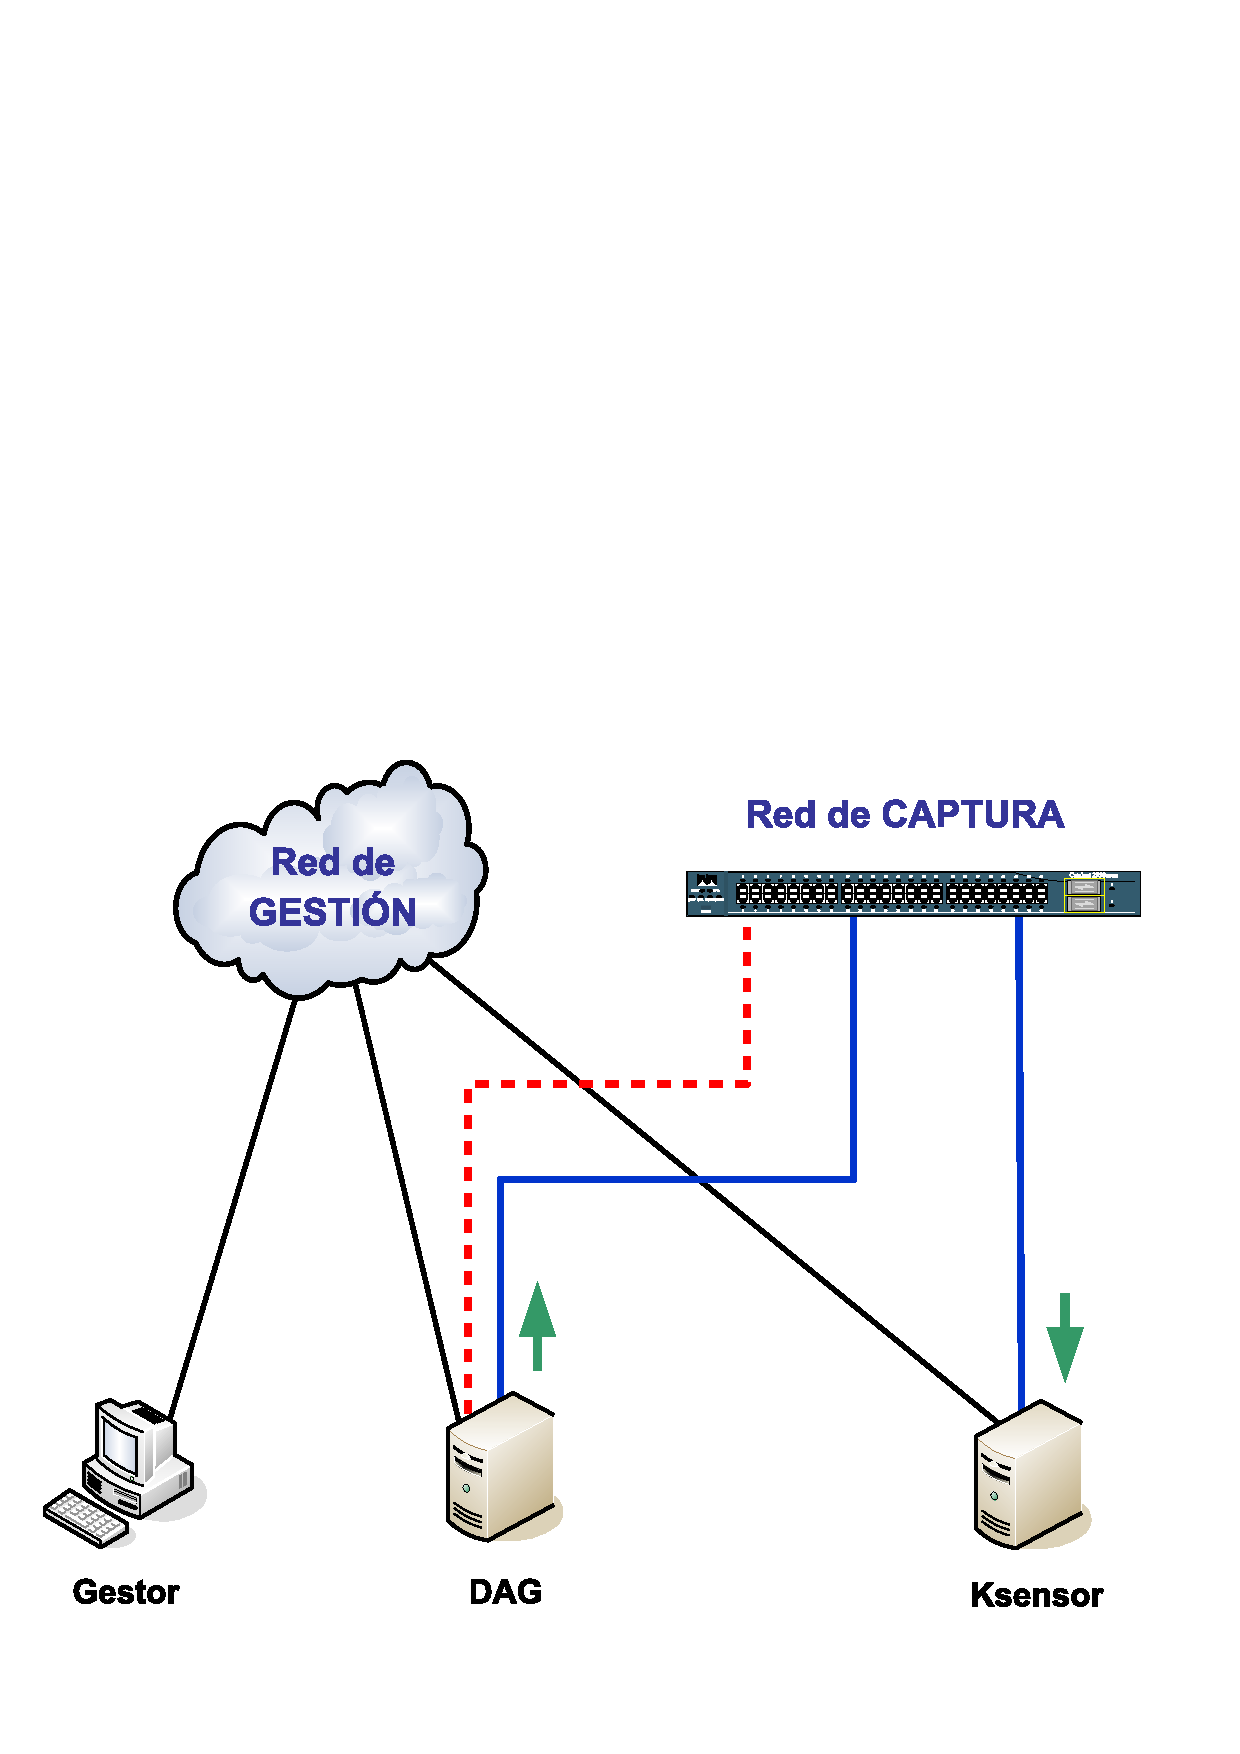
\includegraphics[width=\linewidth]{arquitectura-de-pruebas}
\caption{Arquitectura para la automatizaci�n de pruebas}
\label{fig:arquitectura-de-pruebas}
\end{figure}

El escenario en el que se realizar�n las pruebas comprende dos redes distintas, una de gesti�n y otra de captura. Las redes deben estar separadas, y la red de captura debe contar con un switch intermedio para tener un dispositivo que de una cuenta exacta de los paquetes entregados al receptor.

En los pr�ximos apartados se describir� cada elemento de la arquitectura, trazando las l�neas m�s significativas de su dise�o y funciones. Para ello, en primer lugar se definir�n los elementos l�gicos que act�an en la realizaci�n de las pruebas, que, si bien ya fueron documentados en \cite{AABS05} y \cite{KABO05}, conviene explicar nuevamente.

\section{Elementos l�gicos de la arquitectura}
La arquitectura de pruebas consta, atendiendo a su funcionalidad, de tres elementos l�gicos, que describimos a continuaci�n:
\begin{enumerate}
\item Gestor
\item Agente
\item Demonio
\end{enumerate}

\subsection{Gestor}
El gestor proporciona la interfaz entre el entorno de pruebas y el administrador. As�, el gestor recibe como entrada un fichero XML en el que se le indican las pruebas a realizar, y los par�metros de configuraci�n para cada una. El gestor ejecutar� las pruebas en el mismo orden en el que se hayan definido, reuniendo para cada una los resultados (estad�sticas) que se obtengan.

Para realizar su tarea, el gestor se comunicar� con uno o m�s agentes, indic�ndole a cada uno las acciones que debe realizar, y recogiendo los resultados que se reciban de los mismos. Se trata pues, de una arquitectura cliente/servidor, donde el gestor har� la funci�n de cliente, conect�ndose a uno o varios servidores (agentes).

\subsection{Agente}
El agente es un servidor a la espera de recibir �rdenes desde el gestor, para actuar de la forma que se le indique sobre los demonios de esa m�quina. Un mismo agente puede actuar sobre varios demonios de forma simult�nea. La comunicaci�n entre el agente y los demonios sigue tres fases:

\begin{description}
\item [Inicializaci�n del demonio] El agente se encarga de arrancar el demonio.
\item [Terminaci�n del demonio] La terminaci�n se puede producir por parte del agente o por parte del demonio, en funci�n de si �ste es maestro o esclavo.
\item [Recolecci�n de estad�sticas] El agente recoge las estad�sticas que el demonio ha almacenado durante su ejecuci�n, y se las env�a al gestor.
\end{description}

\subsection{Demonio}
Los demonios son los encargados de realizar las acciones sobre los dispositivos o elementos de la red que se quieren configurar. Un demonio puede realizar cualquier tipo de acci�n, siempre y cuando se ajuste a una interfaz previamente definida para el intercambio de comandos y datos con el agente correspondiente.

Los demonios pueden ser de dos tipos, en funci�n de la relaci�n que mantienen con el agente:

\begin{description}
\item [Maestros] El agente arrancar� estos demonios, pero ser�n ellos los que indiquen cuando han finalizado, en funci�n de lo que tarden en ejecutarse. La duraci�n total de la prueba depender� del tiempo de ejecuci�n de los demonios maestro.
\item [Esclavos] El agente controlar� tanto el arranque como la finalizaci�n de los demonios esclavo. Su finalizaci�n la determinar� el gestor una vez se haya terminado de ejecutar los demonios maestro.
\end{description}

\section{Demonios de la arquitectura}
Para llevar a cabo las pruebas de rendimiento en el sensor, se han creado dos demonios, a saber:

\begin{enumerate}
\item Recolector de estad�sticas
\item Traceador
\end{enumerate}

A continuaci�n se explicar�n las funciones y caracter�sticas de cada uno indicando las consideraciones a tener en cuenta.

\subsection{Recolector de estad�sticas}
El gestor debe poder recolectar las estad�sticas de este m�dulo y resetearlas cuando comience una nueva prueba. Con este fin, se ha dise�ado un demonio que permite controlar y recolectar de forma remota las estad�sticas del m�dulo.

Se ha dise�ado de tal manera que el demonio al activar las estad�sticas las resetee a 0, y que al desactivarlas, tambi�n descargue el m�dulo de su ejecuci�n.

\subsection{Traceador}
En este caso, el gestor debe adem�s de activar y desactivar el m�dulo, guardar todas las trazas de alg�n modo. Para ello se ha dise�ado para que en vez de mandar la informaci�n a trav�s de la salida est�ndar, se mande un fichero generado con el contenido, ya que por las caracter�sticas del m�dulo se sabe que la salida va a ser grande.

\pagenumbering{Roman}

\bibliography{../bibliography}

\printindex

\end{document}
